% OLD
%\documentclass[11pt,compress,t,notes=noshow, aspectratio=169, xcolor=table]{beamer}
% new
\documentclass[10pt,compress,t,notes=noshow, xcolor=table]{beamer}

% OLD
%\usepackage{../../style/lmu-lecture}
% new
\usepackage[]{graphicx}
% graphicx is loaded via lmu-lecture.sty as well
\usepackage[]{color}
% maxwidth is the original width if it is less than linewidth
% otherwise use linewidth (to make sure the graphics do not exceed the margin)
\makeatletter
\def\maxwidth{ %
  \ifdim\Gin@nat@width>\linewidth
    \linewidth
  \else
    \Gin@nat@width
  \fi
}
\makeatother

% ---------------------------------%
% latex-math dependencies, do not remove:
% - mathtools
% - bm
% - siunitx
% - dsfont
% - xspace
% ---------------------------------%

%--------------------------------------------------------%
%       Language, encoding, typography
%--------------------------------------------------------%

\usepackage[english]{babel}
\usepackage[utf8]{inputenc} % Enables inputting UTF-8 symbols
% Standard AMS suite (loaded via lmu-lecture.sty)
\usepackage{amsmath,amsfonts,amssymb}

% Font for double-stroke / blackboard letters for sets of numbers (N, R, ...)
% Distribution name is "doublestroke"
% According to https://mirror.physik.tu-berlin.de/pub/CTAN/fonts/doublestroke/dsdoc.pdf
% the "bbm" package does a similar thing and may be superfluous.
% Required for latex-math
\usepackage{dsfont}

% bbm – "Blackboard-style" cm fonts (https://www.ctan.org/pkg/bbm)
% Used to be in common.tex, loaded directly after this file
% Maybe superfluous given dsfont is loaded
% TODO: Check if really unused?
% \usepackage{bbm}

% bm – Access bold symbols in maths mode - https://ctan.org/pkg/bm
% Required for latex-math, preferred over \boldsymbol
% https://tex.stackexchange.com/questions/3238/bm-package-versus-boldsymbol
\usepackage{bm}

% pifont – Access to PostScript standard Symbol and Dingbats fonts
% Used for \newcommand{\xmark}{\ding{55}, which is never used
% aside from lecture_advml/attic/xx-automl/slides.Rnw
% \usepackage{pifont}

% Quotes (inline and display), provdes \enquote
% https://ctan.org/pkg/csquotes
\usepackage{csquotes}

% Adds arg to enumerate env, technically superseded by enumitem according
% to https://ctan.org/pkg/enumerate
% Replace with https://ctan.org/pkg/enumitem ?
% Even better: enumitem is not really compatible with beamer and breaks all sorts of things
% particularly the enumerate environment. The enumerate package also just isn't required
% from what I can tell so... don't re-add it I guess?
% \usepackage{enumerate}

% Line spacing - provides \singlespacing \doublespacing \onehalfspacing
% https://ctan.org/pkg/setspace
% \usepackage{setspace}

% mathtools – Mathematical tools to use with amsmath
% https://ctan.org/pkg/mathtools?lang=en
% latex-math dependency according to latex-math repo
\usepackage{mathtools}

% Maybe not great to use this https://tex.stackexchange.com/a/197/19093
% Use align instead -- TODO: Global search & replace to check, eqnarray is used a lot
% $ rg -f -u "\begin{eqnarray" -l | grep -v attic | awk -F '/' '{print $1}' | sort | uniq -c
%   13 lecture_advml
%   14 lecture_i2ml
%    2 lecture_iml
%   27 lecture_optimization
%   45 lecture_sl
\usepackage{eqnarray}

% For shaded regions / boxes
% Used sometimes in optim
% https://www.ctan.org/pkg/framed
\usepackage{framed}

%--------------------------------------------------------%
%       Cite button (version 2024-05)
%--------------------------------------------------------%
% Note this requires biber to be in $PATH when running,
% telltale error in log would be e.g. Package biblatex Info: ... file 'authoryear.dbx' not found
% aside from obvious "biber: command not found" or similar.
% Tried moving this to lmu-lecture.sty but had issues I didn't quite understood,
% so it's here for now.

\usepackage{textcase} % for \NoCaseChange
\usepackage{hyperref}

% Only try adding a references file if it exists, otherwise
% this would compile error when references.bib is not found
\IfFileExists{references.bib} {
  \usepackage{usebib}
  \usepackage[backend=biber, style=authoryear]{biblatex}

  \addbibresource{./references.bib}
  \bibinput{references}
}

\newcommand{\citelink}[1]{%
\NoCaseChange{\resizebox{!}{9pt}{\protect\beamergotobutton{\href{\usebibentry{\NoCaseChange{#1}}{url}}{\begin{NoHyper}\cite{#1}\end{NoHyper}}}}}%
}

%--------------------------------------------------------%
%       Displaying code and algorithms
%--------------------------------------------------------%

% Reimplements verbatim environments: https://ctan.org/pkg/verbatim
% verbatim used sed at least once in
% supervised-classification/slides-classification-tasks.tex
% Removed since code should not be put on slides anyway
% \usepackage{verbatim}

% Both used together for algorithm typesetting, see also overleaf: https://www.overleaf.com/learn/latex/Algorithms
% algorithmic env is also used, but part of the bundle:
%   "algpseudocode is part of the algorithmicx bundle, it gives you an improved version of algorithmic besides providing some other features"
% According to https://tex.stackexchange.com/questions/229355/algorithm-algorithmic-algorithmicx-algorithm2e-algpseudocode-confused
\usepackage{algorithm}
\usepackage{algpseudocode}

%--------------------------------------------------------%
%       Tables
%--------------------------------------------------------%

% multi-row table cells: https://www.namsu.de/Extra/pakete/Multirow.html
% Provides \multirow
% Used e.g. in evaluation/slides-evaluation-measures-classification.tex
\usepackage{multirow}

% colortbl: https://ctan.org/pkg/colortbl
% "The package allows rows and columns to be coloured, and even individual cells." well.
% Provides \columncolor and \rowcolor
% \rowcolor is used multiple times, e.g. in knn/slides-knn.tex
\usepackage{colortbl}

% long/multi-page tables: https://texdoc.org/serve/longtable.pdf/0
% Not used in slides
% \usepackage{longtable}

% pretty table env: https://ctan.org/pkg/booktabs
% Is used
% Defines \toprule
\usepackage{booktabs}

%--------------------------------------------------------%
%       Figures: Creating, placing, verbing
%--------------------------------------------------------%

% wrapfig - Wrapping text around figures https://de.overleaf.com/learn/latex/Wrapping_text_around_figures
% Provides wrapfigure environment -used in lecture_optimization
\usepackage{wrapfig}

% Sub figures in figures and tables
% https://ctan.org/pkg/subfig -- supersedes subfigure package
% Provides \subfigure
% \subfigure not used in slides but slides-tuning-practical.pdf errors without this pkg, error due to \captionsetup undefined
\usepackage{subfig}

% Actually it's pronounced PGF https://en.wikibooks.org/wiki/LaTeX/PGF/TikZ
\usepackage{tikz}

% No idea what/why these settings are what they are but I assume they're there on purpose
\usetikzlibrary{shapes,arrows,automata,positioning,calc,chains,trees, shadows}
\tikzset{
  %Define standard arrow tip
  >=stealth',
  %Define style for boxes
  punkt/.style={
    rectangle,
    rounded corners,
    draw=black, very thick,
    text width=6.5em,
    minimum height=2em,
    text centered},
  % Define arrow style
  pil/.style={
    ->,
    thick,
    shorten <=2pt,
    shorten >=2pt,}
}

%--------------------------------------------------------%
%       Beamer setup and custom macros & environments
%--------------------------------------------------------%

% Main sty file for beamer setup (layout, style, lecture page numbering, etc.)
% For long-term maintenance, this may me refactored into a more modular set of .sty files
\usepackage{../../style/lmu-lecture}
% Custom itemize wrappers, itemizeS, itemizeL, etc
\usepackage{../../style/customitemize}
% Custom framei environment, uses custom itemize!
\usepackage{../../style/framei}
% Custom frame2 environment, allows specifying font size for all content
\usepackage{../../style/frame2}
% Column layout macros
\usepackage{../../style/splitV} 

% Used regularly
\let\code=\texttt

% Not sure what/why this does
\setkeys{Gin}{width=0.9\textwidth}

% -- knitr leftovers --
% Used often in conjunction with \definecolor{shadecolor}{rgb}{0.969, 0.969, 0.969}
% Removing definitions requires chaning _many many_ slides, which then need checking to see if output still ok
\definecolor{fgcolor}{rgb}{0.345, 0.345, 0.345}
\definecolor{shadecolor}{rgb}{0.969, 0.969, 0.969}
\newenvironment{knitrout}{}{} % an empty environment to be redefined in TeX

%-------------------------------------------------------------------------------------------------------%
%  Unused stuff that needs to go but is kept here currently juuuust in case it was important after all  %
%-------------------------------------------------------------------------------------------------------%

% \newcommand{\hlnum}[1]{\textcolor[rgb]{0.686,0.059,0.569}{#1}}%
% \newcommand{\hlstr}[1]{\textcolor[rgb]{0.192,0.494,0.8}{#1}}%
% \newcommand{\hlcom}[1]{\textcolor[rgb]{0.678,0.584,0.686}{\textit{#1}}}%
% \newcommand{\hlopt}[1]{\textcolor[rgb]{0,0,0}{#1}}%
% \newcommand{\hlstd}[1]{\textcolor[rgb]{0.345,0.345,0.345}{#1}}%
% \newcommand{\hlkwa}[1]{\textcolor[rgb]{0.161,0.373,0.58}{\textbf{#1}}}%
% \newcommand{\hlkwb}[1]{\textcolor[rgb]{0.69,0.353,0.396}{#1}}%
% \newcommand{\hlkwc}[1]{\textcolor[rgb]{0.333,0.667,0.333}{#1}}%
% \newcommand{\hlkwd}[1]{\textcolor[rgb]{0.737,0.353,0.396}{\textbf{#1}}}%
% \let\hlipl\hlkwb

% \makeatletter
% \newenvironment{kframe}{%
%  \def\at@end@of@kframe{}%
%  \ifinner\ifhmode%
%   \def\at@end@of@kframe{\end{minipage}}%
%   \begin{minipage}{\columnwidth}%
%  \fi\fi%
%  \def\FrameCommand##1{\hskip\@totalleftmargin \hskip-\fboxsep
%  \colorbox{shadecolor}{##1}\hskip-\fboxsep
%      % There is no \\@totalrightmargin, so:
%      \hskip-\linewidth \hskip-\@totalleftmargin \hskip\columnwidth}%
%  \MakeFramed {\advance\hsize-\width
%    \@totalleftmargin\z@ \linewidth\hsize
%    \@setminipage}}%
%  {\par\unskip\endMakeFramed%
%  \at@end@of@kframe}
% \makeatother

% \definecolor{shadecolor}{rgb}{.97, .97, .97}
% \definecolor{messagecolor}{rgb}{0, 0, 0}
% \definecolor{warningcolor}{rgb}{1, 0, 1}
% \definecolor{errorcolor}{rgb}{1, 0, 0}
% \newenvironment{knitrout}{}{} % an empty environment to be redefined in TeX

% \usepackage{alltt}
% \newcommand{\SweaveOpts}[1]{}  % do not interfere with LaTeX
% \newcommand{\SweaveInput}[1]{} % because they are not real TeX commands
% \newcommand{\Sexpr}[1]{}       % will only be parsed by R
% \newcommand{\xmark}{\ding{55}}%

% textpos – Place boxes at arbitrary positions on the LATEX page
% https://ctan.org/pkg/textpos
% Provides \begin{textblock}
% TODO: Check if really unused?
% \usepackage[absolute,overlay]{textpos}

% -----------------------%
% Likely knitr leftovers %
% -----------------------%

% psfrag – Replace strings in encapsulated PostScript figures
% https://www.overleaf.com/latex/examples/psfrag-example/tggxhgzwrzhn
% https://ftp.mpi-inf.mpg.de/pub/tex/mirror/ftp.dante.de/pub/tex/macros/latex/contrib/psfrag/pfgguide.pdf
% Can't tell if this is needed
% TODO: Check if really unused?
% \usepackage{psfrag}

% arydshln – Draw dash-lines in array/tabular
% https://www.ctan.org/pkg/arydshln
% !! "arydshln has to be loaded after array, longtable, colortab and/or colortbl"
% Provides \hdashline and \cdashline
% Not used in slides
% \usepackage{arydshln}

% tabularx – Tabulars with adjustable-width columns
% https://ctan.org/pkg/tabularx
% Provides \begin{tabularx}
% Not used in slides
% \usepackage{tabularx}

% placeins – Control float placement
% https://ctan.org/pkg/placeins
% Defines a \FloatBarrier command
% TODO: Check if really unused?
% \usepackage{placeins}

% Can't find a reason why common.tex is not just part of this file?
% This file is included in slides and exercises

% Rarely used fontstyle for R packages, used only in 
% - forests/slides-forests-benchmark.tex
% - exercises/single-exercises/methods_l_1.Rnw
% - slides/cart/attic/slides_extra_trees.Rnw
\newcommand{\pkg}[1]{{\fontseries{b}\selectfont #1}}

% Spacing helpers, used often (mostly in exercises for \dlz)
\newcommand{\lz}{\vspace{0.5cm}} % vertical space (used often in slides)
\newcommand{\dlz}{\vspace{1cm}}  % double vertical space (used often in exercises, never in slides)
\newcommand{\oneliner}[1] % Oneliner for important statements, used e.g. in iml, algods
{\begin{block}{}\begin{center}\begin{Large}#1\end{Large}\end{center}\end{block}}

% Don't know if this is used or needed, remove?
% textcolor that works in mathmode
% https://tex.stackexchange.com/a/261480
% Used e.g. in forests/slides-forests-bagging.tex
% [...] \textcolor{blue}{\tfrac{1}{M}\sum^M_{m} [...]
% \makeatletter
% \renewcommand*{\@textcolor}[3]{%
%   \protect\leavevmode
%   \begingroup
%     \color#1{#2}#3%
%   \endgroup
% }
% \makeatother


% Defines macros and environments
 
\title{Interpretable Machine Learning}
% \author{LMU}
%\institute{\href{https://compstat-lmu.github.io/lectureml/}{compstat-lmu.github.io/lecture\ml}}
\date{}

\begin{document}

% OLD
%\newcommand{\titlefigure}{figure/2023_paper_skizze_Planted_Tree.jpg}
%\newcommand{\learninggoals}{
%\item Motivation for RPFs
%\item Understand node types and restricting interactions in decision trees
%\item Understand planted trees: non-binary decision trees and inner leaves
%}
%
%\lecturechapter{Random Planted Forests}
%\lecture{Interpretable Machine Learning}
% new
\titlemeta{
Interpretable Models 2
}{
Random Planted Forests
}{
figure/2023_paper_skizze_Planted_Tree.jpg
}{
\item Motivation for RPFs
\item Understand node types and restricting interactions in decision trees
\item Understand planted trees: non-binary decision trees and inner leaves
}


%------------------------------------------------------------------
%------------------------------------------------------------------

\begin{frame}{Random Planted Forests (RPF) % OLD
%\citebutton{Hiabu et al. 2023}{https://arxiv.org/abs/2012.14563}
% new
\furtherreading{Hiabu_et_al_2023}}

\textbf{Goal:} Create a powerful tree ensemble, but still interpretable

\textbf{Idea:}
\begin{itemize}
    \item GAMs easily interpretable, because no interaction $\leadsto$ Plot 1D functions
    
    \begin{columns}[T, totalwidth=\textwidth]
    \begin{column}{0.5\textwidth}
    $$
    \hat{f}(x) = \theta_0 + f_1(x_{1}) + f_2(x_{2}) + \ldots + f_p(x_{p}),
    $$
    \end{column}
    \hspace*{0.4cm}\hfill
    \centering
    \begin{column}{0.5\textwidth}
    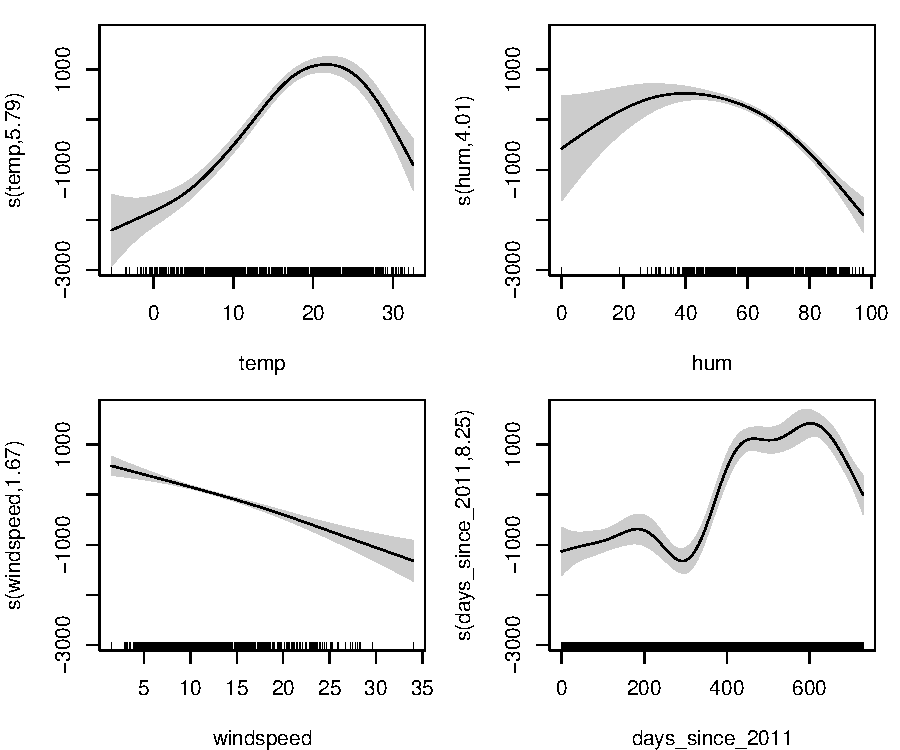
\includegraphics[width = .4\textwidth]{figure/gam_effects.pdf}
    \end{column}
    \end{columns}
    
    \item Same for function containing interactions between max. 2 features 
    \\ $\leadsto$ function of 2 features, Plot 2D functions (i.e. 3D plot)

    $$
    \hat{f}(x) = \theta_0 + f_1(x_{1}) + f_2(x_{2}) + \ldots + f_p(x_{p}) + f_{1,2}(x_{1}, x_{2}) + \ldots + f_{1,p}(x_{1}, x_{p}) + \ldots + f_{p-1,p}(x_{p-1}, x_{p}),
    $$

    $\leadsto$ Visualize single functions $f_1, f_2, f_{1,2}(x_{1}, x_{2}), f_{1,3}(x_{1}, x_{3}) \ldots$

    % TODO Also figures ?
    
\end{itemize}

$\Rightarrow$ Interpretability possible via restricting degree of interactions

\textbf{Problem:} How to know degree of interactions?

\textbf{Solution:} Easy to determine for trees / tree ensembles!

\end{frame}

\begin{frame}{RPF: Determine interaction type in trees}

Define the \textit{interaction type $t$} of a node as the subset of features involved in constructing this node.

\textbf{Example:}

\begin{center}
    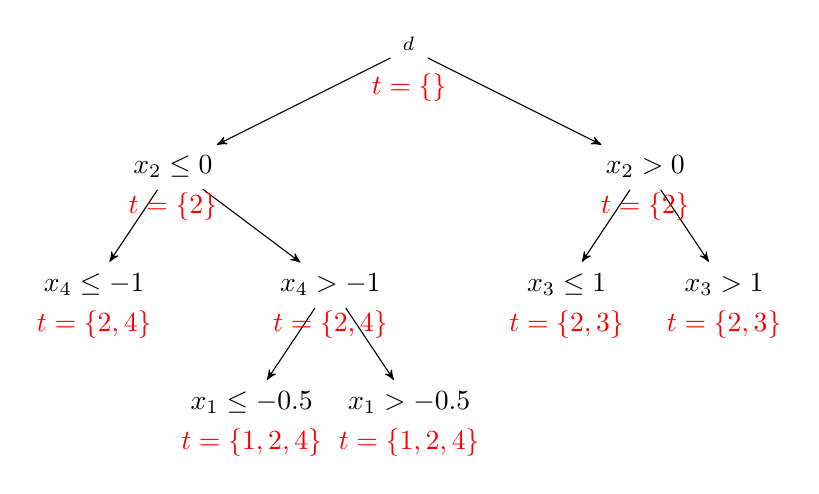
\begin{tikzpicture}[
    node/.style = {scale=1},
    scale = 1
    ]
        
        % \node[node] at (0,0)(root){\(x_2 \leq 0\)};
        % 
        % \node[node] at (3,-1)(right_child){\(x_3 \leq 1\)};
        % \node[node] at (4,-2)(rightright_grandchild){$0.6$};
        % \node[node] at (2,-2)(rightleft_grandchild){\(-0.3\)};
        % 
        % \node[node] at (-3,-1)(left_child){\(x_4 \leq -1\)};
        % \node[node] at (-4,-2)(leftleft_grandchild){$0.2$};
        % \node[node] at (-2,-2)(leftright_grandchild){\(x_1 \leq -0.5\)};
        % 
        % \node[node] at (-2.5,-3)(low_child_1){$-0.1$};
        % \node[node] at (-1.5,-3)(low_child_2){$0.7$};
        
        \node[node] at (0,2)(root){\(\R^d\)};
        
        \node[node] at (3,.5)(right_child){\(x_2 > 0\)};
        \node[node] at (4,-1)(rightright_grandchild){$x_3 > 1$};
        \node[node] at (2,-1)(rightleft_grandchild){\(x_3 \leq 1\)};
        
        \node[node] at (-3,.5)(left_child){\(x_2 \leq 0\)};
        \node[node] at (-4,-1)(leftleft_grandchild){$x_4 \leq -1$};
        \node[node] at (-1,-1)(leftright_grandchild){\(x_4 > -1\)};
        
        \node[node] at (-2,-2.5)(low_child_1){$x_1 \leq -0.5$};
        \node[node] at (-0,-2.5)(low_child_2){$x_1 > -0.5$};

        \draw[->, shorten >= 1pt, shorten <= 1pt] (root) -- (left_child);
        \draw[->, shorten >= 1pt, shorten <= 1pt] (root) -- (right_child);
        \draw[->, shorten >= 1pt, shorten <= 1pt] (left_child) -- (leftleft_grandchild);
        \draw[->, shorten >= 1pt, shorten <= 1pt] (left_child) -- (leftright_grandchild);
        \draw[->, shorten >= 1pt, shorten <= 1pt] (right_child) -- (rightright_grandchild);
        \draw[->, shorten >= 1pt, shorten <= 1pt] (right_child) -- (rightleft_grandchild);
        
        \draw[->, shorten >= 1pt, shorten <= 1pt] (leftright_grandchild) -- (low_child_1);
        \draw[->, shorten >= 1pt, shorten <= 1pt] (leftright_grandchild) -- (low_child_2);

        \only<2>{
        \node[node, color=red] at (0,1.5)(root_type){$t=\{\}$};
        
        \node[node, color=red] at (3,0)(right_child_type){$t=\{2\}$};
        \node[node, color=red] at (4,-1.5)(rightright_grandchild_type){$t=\{2,3\}$};
        \node[node, color=red] at (2,-1.5)(rightleft_grandchild_type){$t=\{2,3\}$};
        
        \node[node, color=red] at (-3,0)(left_child_type){$t=\{2\}$};
        \node[node, color=red] at (-4,-1.5)(leftleft_grandchild_type){$t=\{2,4\}$};
        \node[node, color=red] at (-1,-1.5)(leftright_grandchild_type){$t=\{2,4\}$};
        
        \node[node, color=red] at (-2,-3)(low_child_1_type){$t=\{1,2,4\}$};
        \node[node, color=red] at (0,-3)(low_child_2_type){$t=\{1,2,4\}$};
        % \draw (-2,-3.3) ellipse (1.1cm and 0.6cm);
        % \draw (0,0) ellipse (2cm and 1cm);
        }

        
    \end{tikzpicture}
\end{center}

\only<2>{
$\Rightarrow$ Degree of interaction in each node is \(|t|\).
}
    
\end{frame}

\begin{frame}{RPF: bounded interaction order + Planted trees}

    Goal: restrict this interaction degree
    
    $\leadsto$ In RPFs: 

    \begin{itemize}
        \item Always keep track of interaction type in each node
        
        \item For each new split, make sure max. degree of interactions is not exceeded $\Rightarrow$ When max. number of feat reached, no new feat are allowed
    \end{itemize}

    \textbf{Problem: } For small interaction order, single trees quickly limited

    \begin{itemize}
        \item E.g. interaction order 1: Every tree only one feature
        \item[$\Rightarrow$] Many trees needed for more complex model
    \end{itemize}

    \textbf{Idea:} Allow inner nodes to split again

    Define \textit{Planted Trees}: Decision trees where each inner nodes can be \textit{leaves}:
    \begin{itemize}
        \item Add prediction to final output
        \item Can be split again $\Rightarrow$ several splits possible
    \end{itemize}
    
\end{frame}

% \begin{frame}{RPF: Example}

%     \begin{figure}[h]
%         \centering
%         % \vspace{-10pt} % Note that this is only to ensure a normal, not to big margin around the figure
%         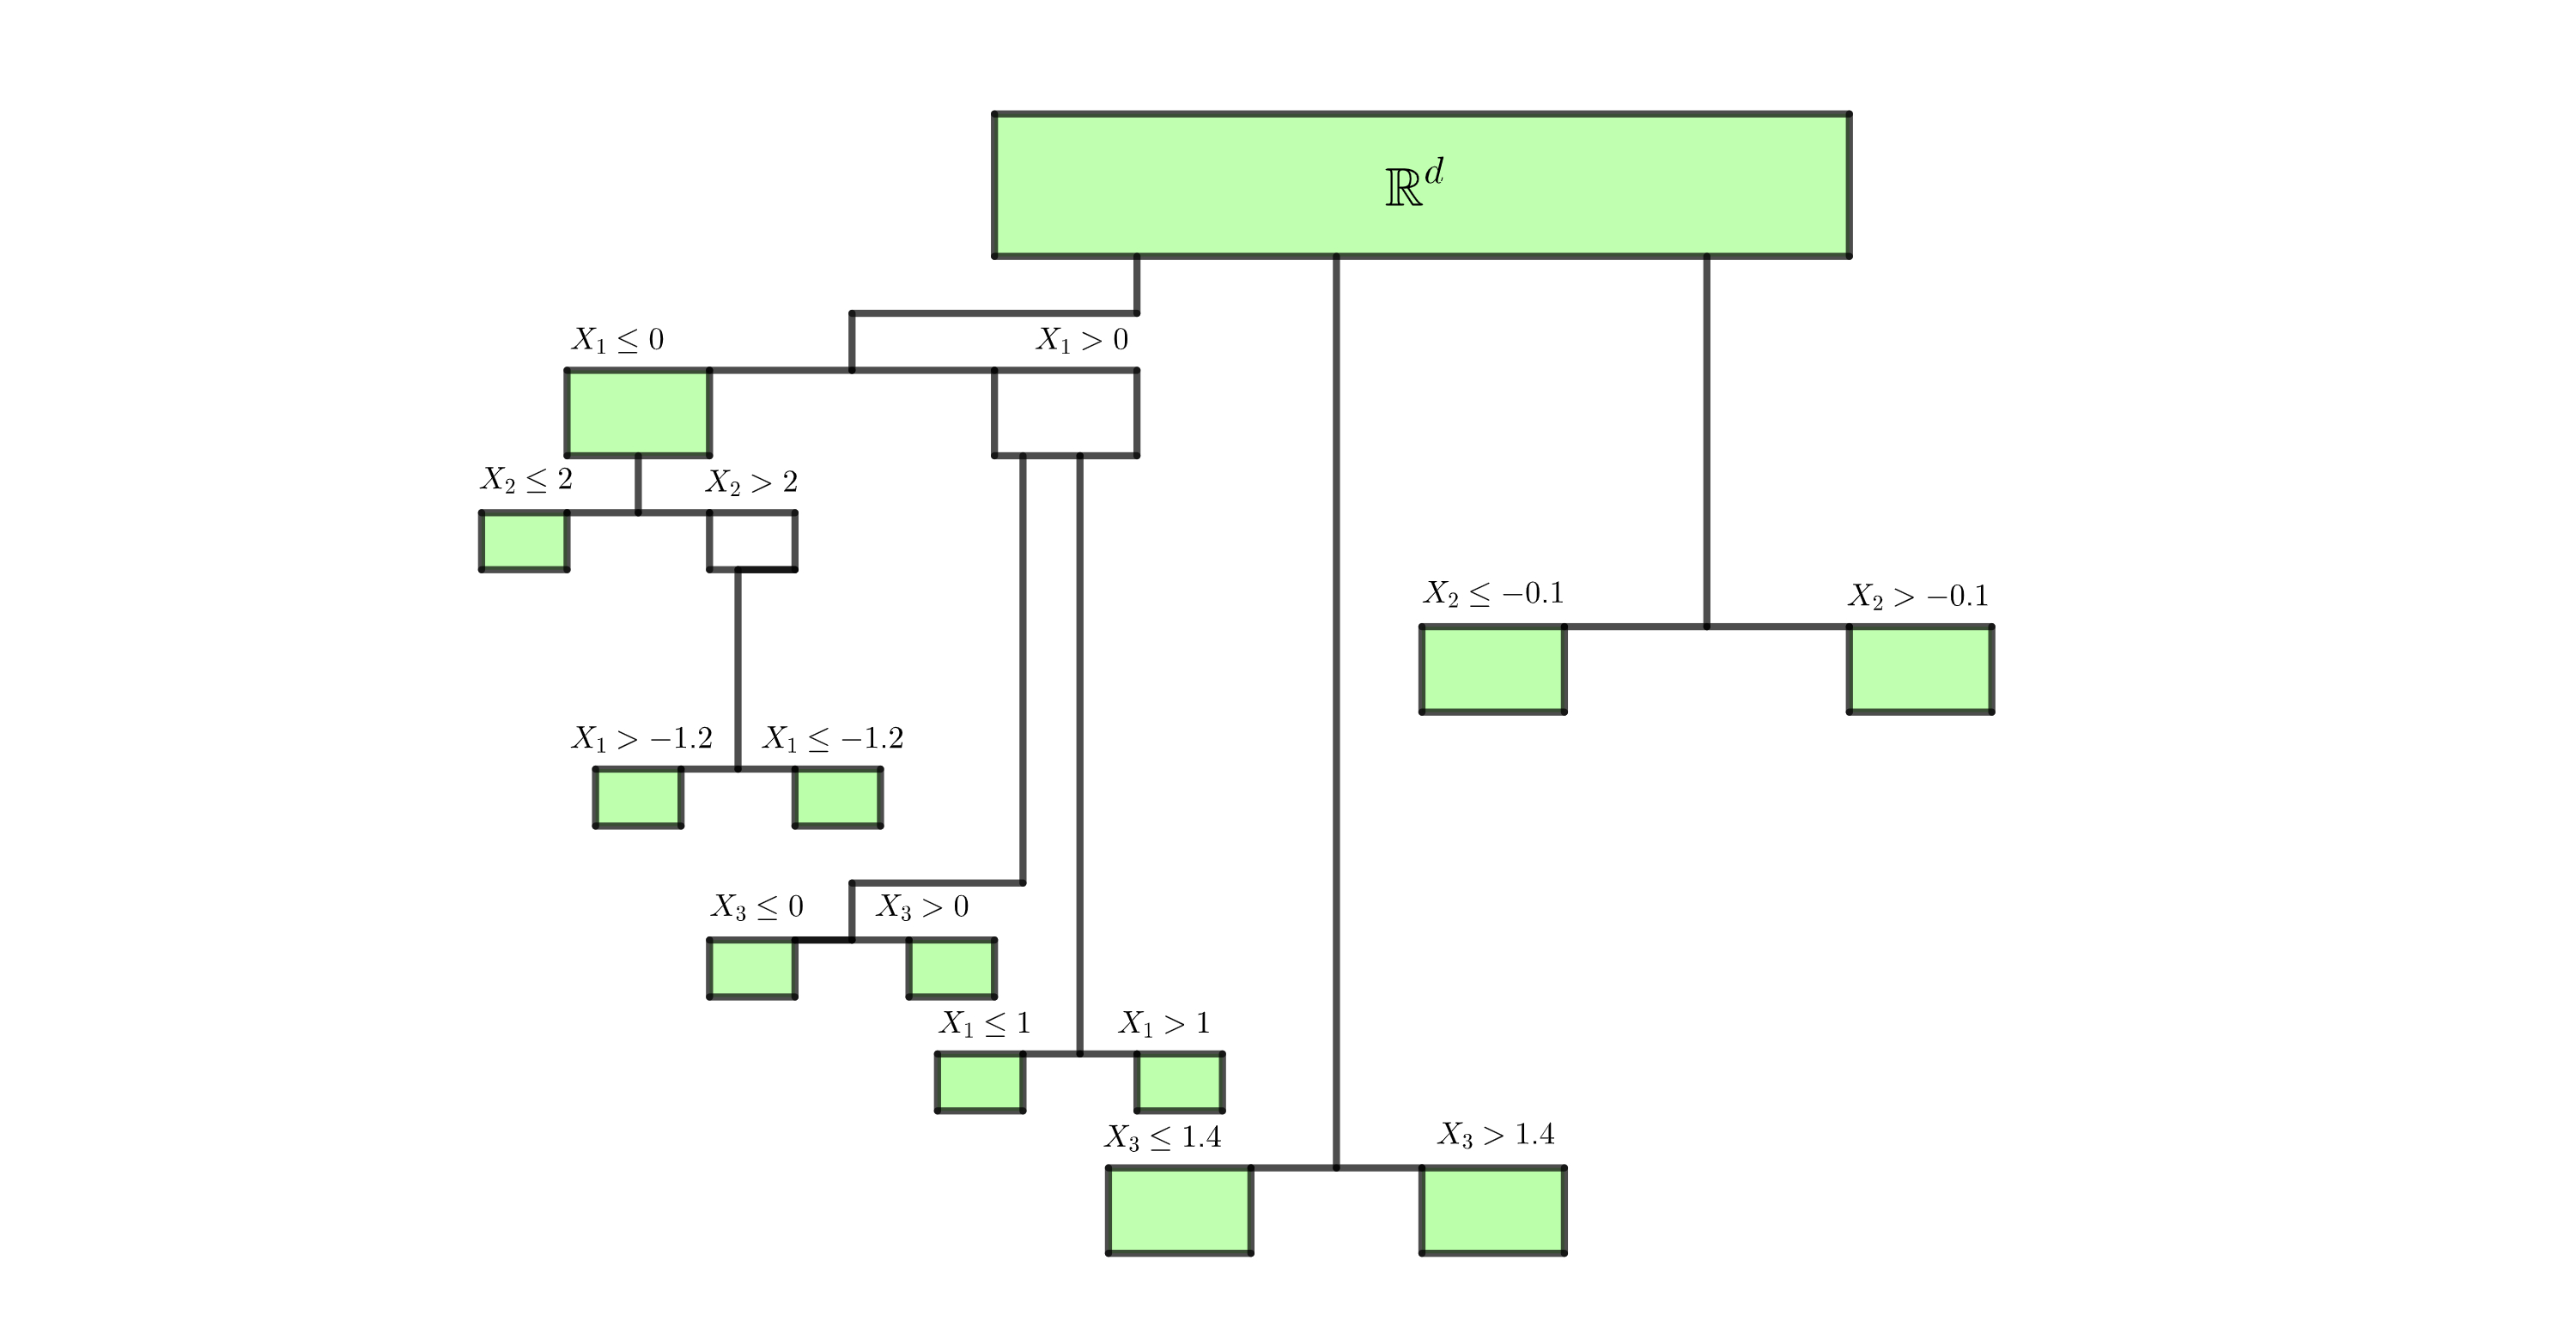
\includegraphics[width=1.1\linewidth]{figure/2023_paper_skizze_Planted_Tree.jpg}
%         % \vspace{-10pt}
%         \caption{Example of a single fully grown planted tree}
%         \label{fig:Planted_Tree_example_paper}
%     \end{figure}

% \end{frame}

\begin{frame}{RPF: Example}

\begin{center}
    \begin{figure}[h]
    
    \begin{tikzpicture}[
    node/.style = {scale=.5},
    scale = 1
    ]
        \node[anchor=south west,inner sep=0] (image) at (0,0) {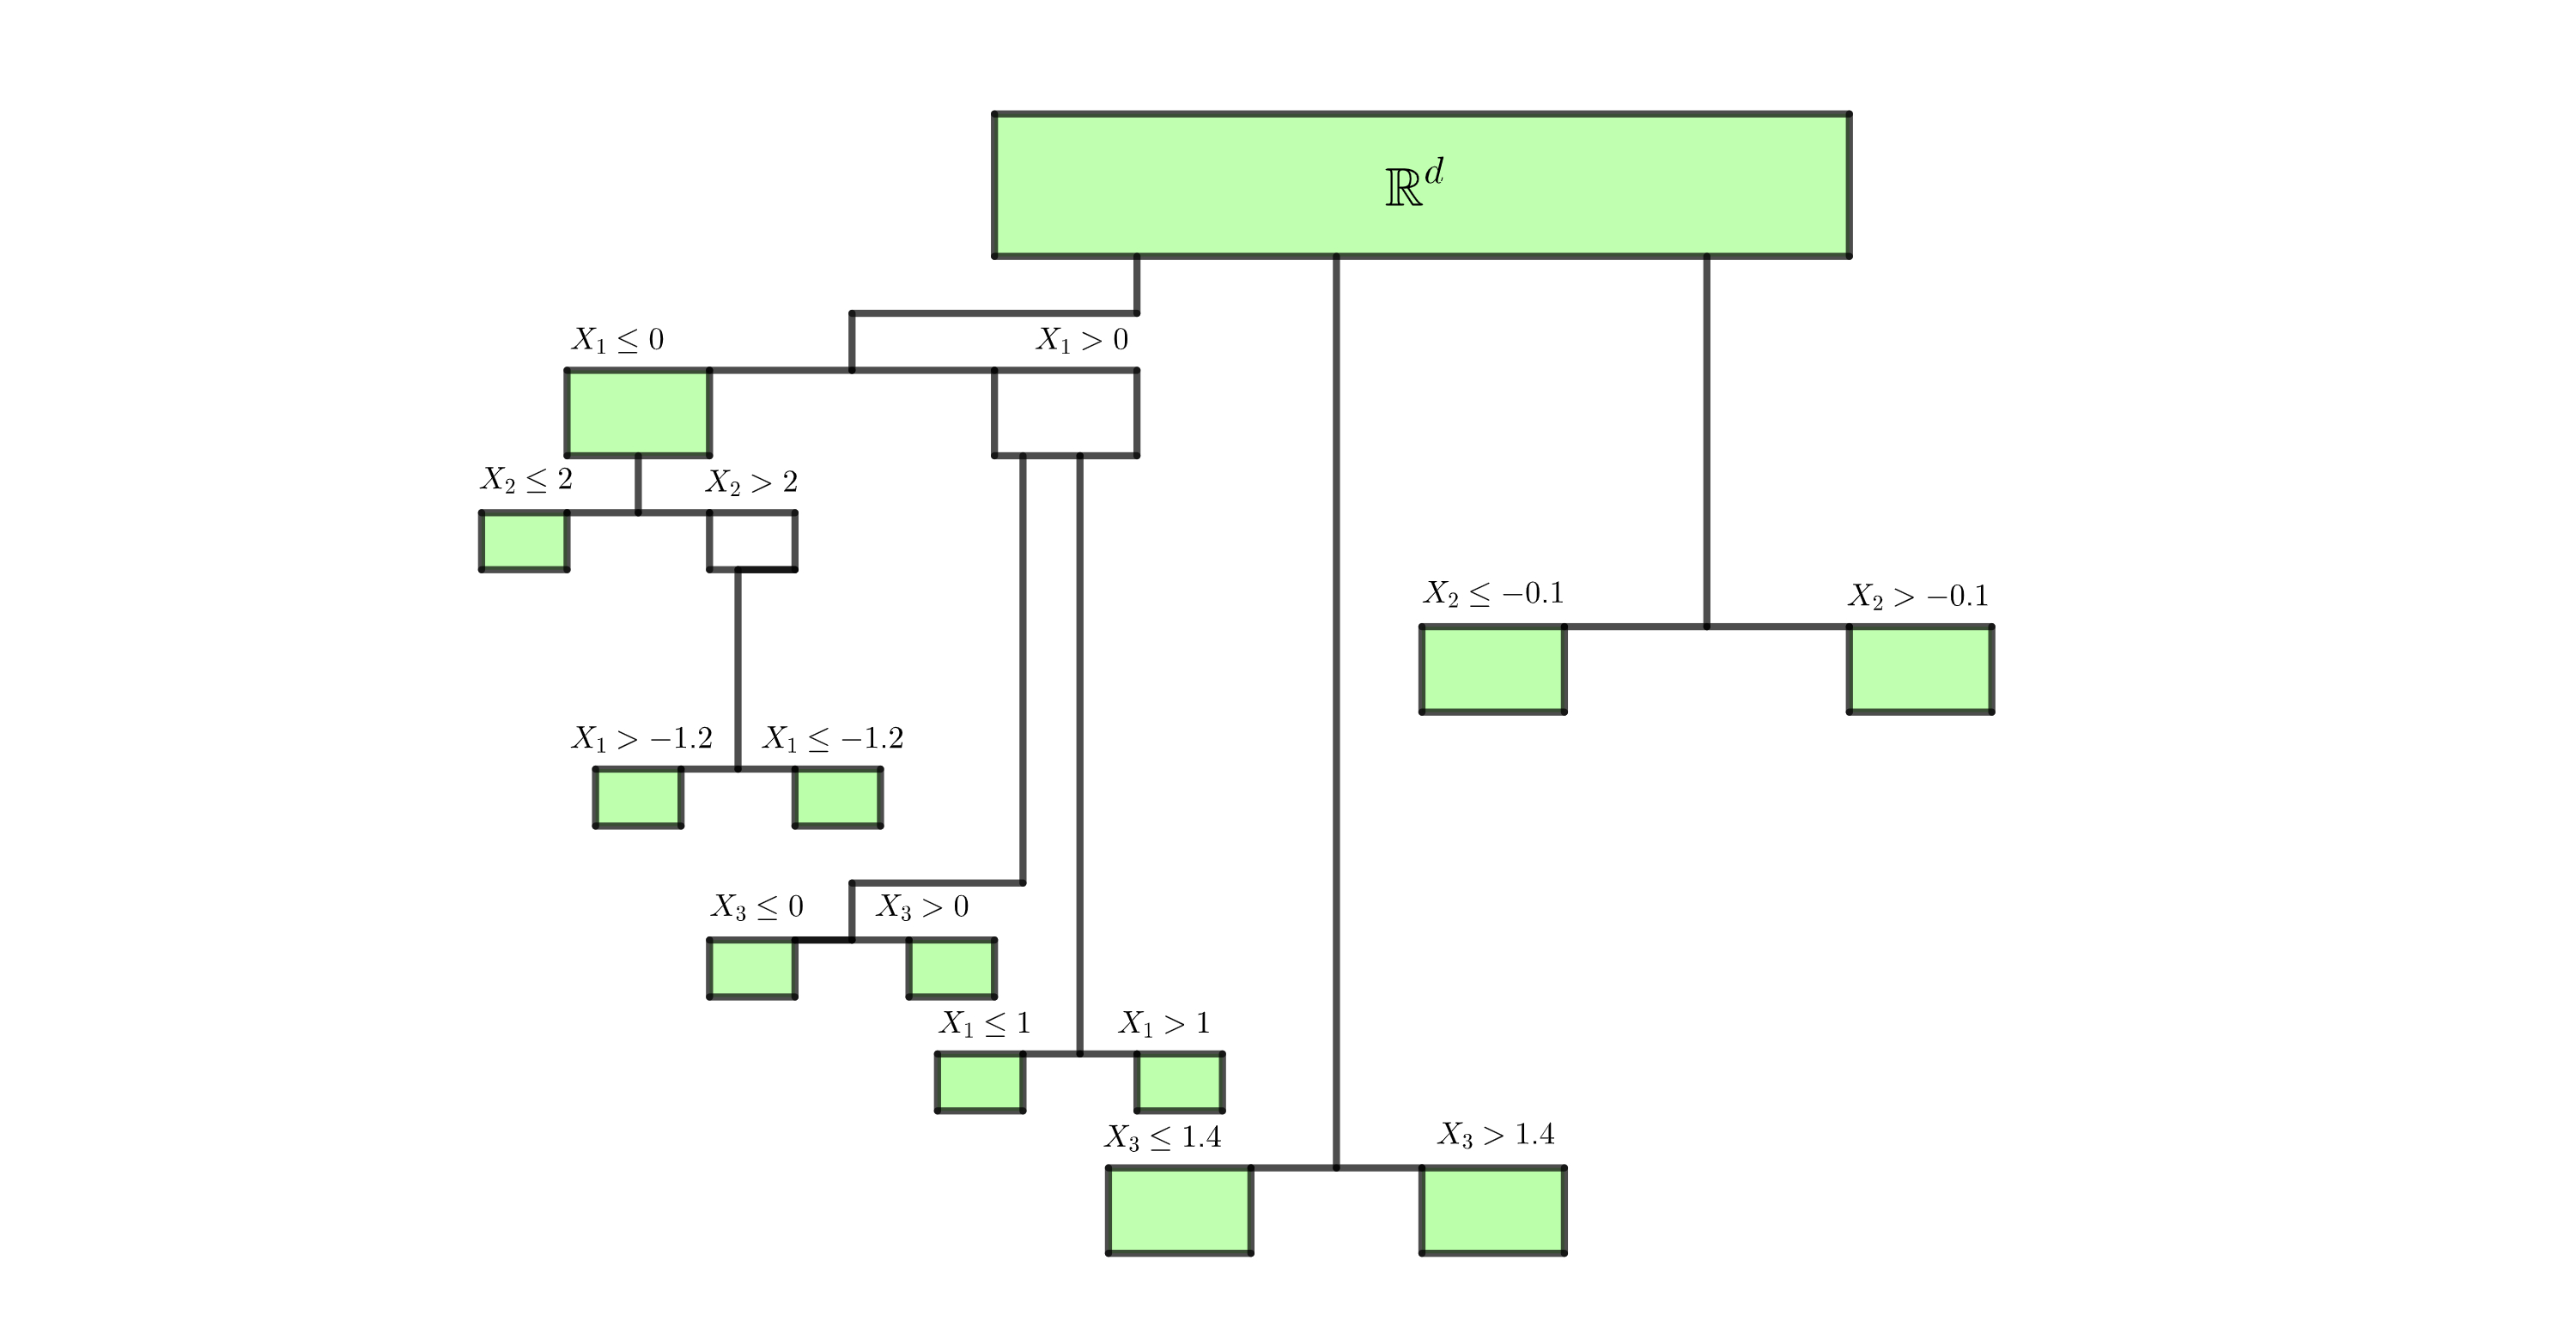
\includegraphics[width=1.1\linewidth]{figure/2023_paper_skizze_Planted_Tree.jpg}};
        
        \only<2>{
        \node[node, color=red] at (8,6)(root_type){$t=\{\}$};
        
        \node[node, color=red] at (3.35,4.8)(leftleft_type){$\{1\}$};
        \node[node, color=red] at (5.55,4.8)(leftright_type){$\{1\}$};
        
        \node[node, color=red] at (3.95,4.1)(leftleft_right_type){$\{1,2\}$};
        \node[node, color=red] at (2.75,4.1)(leftleft_left_type){$\{1,2\}$};
        
        \node[node, color=red] at (3.35,2.8)(leftleft_right_left_type){$\{1,2\}$};
        \node[node, color=red] at (4.35,2.8)(leftleft_right_right_type){$\{1,2\}$};
        
        \node[node, color=red] at (3.95,1.9)(leftright_leftleft_type){$\{1,3\}$};
        \node[node, color=red] at (4.95,1.9)(leftright_leftright_type){$\{1,3\}$};
        
        % \node[node, color=red] at (5,1)(left_right_type_dummy){$\{1\}$};
        \node[node, color=red] at (5.15,1.25)(leftright_rightleft_type){$\{1\}$};
        \node[node, color=red] at (6.15,1.25)(leftright_rightright_type){$\{1\}$};
        
        \node[node, color=red] at (7.75,.65)(midright_type){$\{3\}$};
        \node[node, color=red] at (6.15,.65)(midleft_type){$\{3\}$};
        }
        
    \end{tikzpicture}
    
    \caption{Example of a single fully grown planted tree, green nodes: ``leaves''}
    \label{fig:Planted_Tree_example_paper}
    \end{figure}

\end{center}
    
\end{frame}

\begin{frame}{RPF: Algo}

\begin{itemize}
    \item Max. interaction degree is a hyperparameter
    \item Total number of trees is a hyperparameter
    \item End growing tree after max. total number of splits instead of max. depth \\
    (min. number of samples also possible, but then higher nodes would split too often)
    \item Randomization as in Random Forests:
    \begin{itemize}
        \item Only optimize over subset of features, randomly chosen
        \item Only optimize over subset of possible split values
    \end{itemize}
    \item Make an inner leaf an inner node (i.e. delete ``leaf'' property), if it has children with the same type
\end{itemize}
    
\end{frame}

\begin{frame}{RPF: Example results and interpretation}
    
\end{frame}

\begin{frame}{RPF: Conclusion}
    
\end{frame}

\endlecture
\end{document}